\chapter{\ifenglish Introduction\else บทนำ\fi}

\section{\ifenglish Project rationale\else ที่มาของโครงงาน\fi}

\par
ปัจจุบัน ระบบห่วงโซ่อุปทานมีบทบาทสำคัญในการขนส่งสินค้า โดยเฉพาะสินค้าที่ต้องควบคุมอุณหภูมิ เช่น อาหารแช่แข็ง ซึ่งจำเป็นต้องได้รับการดูแลอย่างเข้มงวดตลอดกระบวนการขนส่ง เพื่อป้องกันการเสื่อมสภาพของสินค้า อย่างไรก็ตาม ระบบห่วงโซ่อุปทานแบบดั้งเดิมยังคงเผชิญกับปัญหาหลายประการ เช่น การขาดความโปร่งใสในการตรวจสอบย้อนกลับ การบันทึกข้อมูลที่ไม่มีประสิทธิภาพ และการรายงานความผิดปกติที่ล่าช้า ซึ่งอาจส่งผลให้สินค้าได้รับความเสียหายและก่อให้เกิดความสูญเสียทางเศรษฐกิจ

เทคโนโลยีบล็อกเชน (Blockchain) และอินเทอร์เน็ตของสรรพสิ่ง (Internet of Things: IoT)
สามารถช่วยแก้ไขปัญหาดังกล่าวได้ โดยบล็อกเชนทำหน้าที่เป็นระบบจัดเก็บข้อมูลแบบกระจายศูนย์ 
(Decentralized Ledger) ซึ่งมีความปลอดภัยสูงและสามารถตรวจสอบย้อนกลับข้อมูลได้อย่างโปร่งใส
ข้อมูลเกี่ยวกับอุณหภูมิและสถานะของสินค้าตลอดเส้นทางขนส่งจะถูกบันทึกลงในบล็อกเชน และไม่สามารถ
เปลี่ยนแปลงหรือปลอมแปลงได้โดยไม่ได้รับอนุญาต ขณะเดียวกัน อินเทอร์เน็ตของสรรพสิ่งมีบทบาทสำคัญใน
การเก็บรวบรวมข้อมูลแบบเรียลไทม์ผ่านเซ็นเซอร์ที่ติดตั้งอยู่ในระบบขนส่ง ซึ่งช่วยให้สามารถติดตามและเฝ้าระวังอุณหภูมิของสินค้าได้อย่างต่อเนื่อง หากตรวจพบอุณหภูมิที่ผิดปกติ ระบบสามารถแจ้งเตือนอัตโนมัติไปยังผู้ที่เกี่ยวข้องเพื่อดำเนินการแก้ไขได้ทันที
\par
ด้วยเหตุนี้ โครงการนี้จึงมุ่งเน้นการพัฒนาและประยุกต์ใช้เทคโนโลยีบล็อกเชนและอินเทอร์เน็ตของสรรพสิ่ง
เพื่อบริหารจัดการห่วงโซ่อุปทานของอาหารแช่แข็ง โดยมีเป้าหมายเพื่อเพิ่มความโปร่งใสของข้อมูล ลดความสูญเสียของสินค้า และสร้างมาตรฐานใหม่ในการขนส่งสินค้าที่ต้องควบคุมอุณหภูมิให้มีประสิทธิภาพยิ่งขึ้น


\section{\ifenglish Objectives\else วัตถุประสงค์ของโครงงาน\fi}
\begin{enumerate}
    \item เพื่อพัฒนาแพลตฟอร์มที่ใช้บล็อกเชน (Blockchain) และอินเทอร์เน็ตของสรรพสิ่ง (IoT) ในการติดตามและบันทึกข้อมูลอุณหภูมิของอาหารแช่แข็งแบบเรียลไทม์
    \item เพื่อออกแบบและพัฒนาระบบที่สามารถแจ้งเตือนอัตโนมัติเมื่ออุณหภูมิของสินค้าอยู่นอกช่วงที่กำหนด
    \item \sloppy เพื่อสร้างระบบที่สามารถตรวจสอบย้อนกลับข้อมูลของอาหารแช่แข็งตลอดซัพพลายเชน (Supply Chain) ได้อย่างโปร่งใสและปลอดภัย
    \item เพื่อลดการสูญเสียของอาหารแช่แข็งอันเนื่องมาจากอุณหภูมิที่ไม่เหมาะสมระหว่างการขนส่ง
    \item เพื่อศึกษาและทดสอบประสิทธิภาพของระบบบล็อกเชน (Blockchain) และอินเทอร์เน็ตของสรรพสิ่ง (IoT) ในการปรับปรุงกระบวนการจัดการซัพพลายเชน (Supply Chain) ของอาหารแช่แข็ง
\end{enumerate}

\section{\ifenglish Project scope\else ขอบเขตของโครงงาน\fi}

\subsection{\ifenglish Hardware scope\else ขอบเขตด้านฮาร์ดแวร์\fi}
\sloppy
ในด้านฮาร์ดแวร์ โครงงานนี้จะเน้นการพัฒนาและติดตั้งอุปกรณ์ที่ใช้ในการตรวจจับอุณหภูมิของอาหารแช่แข็ง
ตลอดการขนส่ง โดยจะใช้เซ็นเซอร์อินเทอร์เน็ตของสรรพสิ่ง (IoT) ที่สามารถเก็บข้อมูลอุณหภูมิแบบเรียล
ไทม์และส่งข้อมูลเหล่านี้ไปยังระบบคลาวด์หรือบล็อกเชน (Blockchain) สำหรับการจัดเก็บและตรวจสอบ
ข้อมูล เซ็นเซอร์ที่ใช้จะต้องมีความแม่นยำสูง สามารถทำงานได้ในอุณหภูมิที่ต่ำ และเชื่อมต่อกับเครือข่ายอินเทอร์เน็ตของสรรพสิ่ง (IoT) ได้อย่างมีประสิทธิภาพ ซึ่งระบบเครือข่ายจะรองรับการส่งข้อมูลจาก
เซ็นเซอร์ไปยังเซิร์ฟเวอร์หลักเพื่อการประมวลผลและการบันทึกลงในบล็อกเชน (Blockchain)

\subsection{\ifenglish Software scope\else ขอบเขตด้านซอฟต์แวร์\fi}
\sloppy
ในด้านซอฟต์แวร์ โครงงานนี้จะพัฒนาระบบที่สามารถบันทึกข้อมูลการขนส่งและอุณหภูมิของสินค้าแบบเรียลไทม์โดยใช้ Blockchain ซึ่งจะทำหน้าที่เป็นระบบฐานข้อมูลที่มีความปลอดภัยสูงและไม่สามารถปลอมแปลงข้อมูลได้ ระบบจะสามารถบันทึกการเปลี่ยนแปลงของอุณหภูมิที่เกิดขึ้นระหว่างการขนส่ง โดยข้อมูลทุกชนิดจะถูกจัดเก็บใน Blockchain พร้อมกับข้อมูลเกี่ยวกับตำแหน่งของสินค้าและสถานะการขนส่ง การใช้ Blockchain ยังจะช่วยให้สามารถตรวจสอบย้อนกลับข้อมูลการขนส่งและการดูแลสินค้าผ่านระบบแบบกระจายศูนย์ได้อย่างโปร่งใสและปลอดภัย สำหรับระบบการแจ้งเตือนอัตโนมัติ จะถูกพัฒนาขึ้นเพื่อส่งข้อความแจ้งเตือนเมื่ออุณหภูมิของสินค้าอยู่นอกช่วงที่กำหนดไว้ ระบบจะแจ้งเตือนผู้ที่เกี่ยวข้องเพื่อให้ดำเนินการแก้ไขได้ทันที หากตรวจพบการผิดปกติในการขนส่ง นอกจากนี้ยังจะมีการพัฒนาแอปพลิเคชันสำหรับผู้ใช้งานที่สามารถติดตามสถานะของการขนส่งและการบันทึกข้อมูลอุณหภูมิได้จากทุกที่ผ่านอุปกรณ์ที่เชื่อมต่ออินเทอร์เน็ต

\section{\ifenglish Expected outcomes\else ประโยชน์ที่ได้รับ\fi}
\sloppy
\begin{enumerate}
    \item ช่วยให้สามารถติดตามอุณหภูมิของอาหารแช่แข็งในระหว่างการขนส่งแบบเรียลไทม์ และสามารถแจ้งเตือนเมื่ออุณหภูมิของสินค้าผิดปกติ ทำให้สามารถดำเนินการแก้ไขได้ทันที ซึ่งจะช่วยป้องกันการเสื่อมสภาพของสินค้าและลดการสูญเสียทางเศรษฐกิจจากการขนส่งที่ไม่เหมาะสม
    \item การใช้บล็อกเชน (Blockchain) ช่วยให้ข้อมูลเกี่ยวกับอุณหภูมิและสถานะของสินค้าในระหว่างการขนส่งถูกบันทึกอย่างโปร่งใสและไม่สามารถปลอมแปลงได้ ซึ่งทำให้ผู้ที่เกี่ยวข้องสามารถตรวจสอบย้อนกลับข้อมูลได้อย่างปลอดภัยและเชื่อถือได้
    \item ระบบสามารถแจ้งเตือนอัตโนมัติเมื่ออุณหภูมิของสินค้าอยู่นอกช่วงที่กำหนด ทำให้สามารถดำเนินการแก้ไขได้ทันที ลดความเสี่ยงในการสูญเสียสินค้าและเพิ่มประสิทธิภาพในการขนส่ง
    \item การใช้เทคโนโลยีบล็อกเชน (Blockchain) และอินเทอร์เน็ตของสรรพสิ่ง (IoT) ช่วยในการจัดเก็บและติดตามข้อมูลแบบอัตโนมัติ ลดต้นทุนในการขนส่งและการจัดการซัพพลายเชนได้อย่างมีประสิทธิภาพ และสามารถปรับปรุงกระบวนการทำงานในองค์กรได้
    \item สร้างมาตรฐานใหม่ในการขนส่งอาหารแช่แข็ง โดยมีการใช้เทคโนโลยีขั้นสูงในการติดตามและควบคุมอุณหภูมิของสินค้า ช่วยยกระดับคุณภาพการขนส่งในอุตสาหกรรมนี้ให้มีความน่าเชื่อถือและมีประสิทธิภาพมากยิ่งขึ้น
\end{enumerate}

\section{\ifenglish Technology and tools\else เทคโนโลยีและเครื่องมือที่ใช้\fi}

\subsection{\ifenglish Hardware technology\else เทคโนโลยีด้านฮาร์ดแวร์\fi}
\subsubsection{บอร์ดคิดไบร์ท (KidBright Board)}
\textbf{เหตุผลที่เลือกใช้:}
\begin{itemize}
    \item เป็นเครื่องมือสำหรับการเรียนรู้ด้านอินเทอร์เน็ตของสรรพสิ่ง (Internet of Things: IoT) โดยเฉพาะ ทำให้เหมาะสมสำหรับการศึกษาพื้นฐานการเขียนโปรแกรมและพัฒนาอุปกรณ์ IoT ที่สามารถนำไปประยุกต์ใช้ในโครงการได้
    \item มีความสะดวกต่อการใช้งานและเหมาะสำหรับโครงการขนาดเล็ก โดยสามารถเริ่มต้นใช้งานได้อย่างรวดเร็ว จึงเหมาะสำหรับการพัฒนาเซ็นเซอร์เพื่อตรวจสอบอุณหภูมิในโครงการนี้
    \item มีต้นทุนต่ำ ทำให้เหมาะสมสำหรับการทดลองและพัฒนาในระดับต้นหรือการสร้างต้นแบบ (Prototype)
    \item รองรับการเชื่อมต่อกับอุปกรณ์ IoT และเซ็นเซอร์ต่าง ๆ ซึ่งช่วยให้สามารถเก็บข้อมูลอุณหภูมิได้แบบเรียลไทม์
\end{itemize}


\subsubsection{เซ็นเซอร์วัดอุณหภูมิแบบดิจิทัล ดีเอส 18 บี 20 (DS18B20 Sensor)}
\textbf{เหตุผลที่เลือกใช้:}
\begin{itemize}
    \item รองรับการวัดอุณหภูมิในช่วงกว้าง ตั้งแต่ -55\textdegree C ถึง +125\textdegree C ซึ่งสามารถครอบคลุมช่วงอุณหภูมิที่ใช้ในกระบวนการขนส่งอาหารแช่แข็งได้เป็นอย่างดี
    \item มีความแม่นยำสูง โดยมีค่าความคลาดเคลื่อนเพียง $\pm$ 0.5\textdegree C ในช่วงอุณหภูมิระหว่าง -10\textdegree C ถึง +85\textdegree C ซึ่งเหมาะสมสำหรับการควบคุมอุณหภูมิของอาหารแช่แข็งที่ต้องรักษาอุณหภูมิให้อยู่ในช่วงที่กำหนด
    \item รองรับการเชื่อมต่อแบบวัน-ไวร์ (1-Wire) โดยใช้สายสัญญาณเพียงเส้นเดียวสำหรับการรับส่งข้อมูล ซึ่งช่วยลดความซับซ้อนของการเดินสายไฟและการติดตั้ง
\end{itemize}


\subsection{\ifenglish Software technology\else เทคโนโลยีด้านซอฟต์แวร์\fi}
\subsubsection{รีแอกต์ (React)}
\textbf{เหตุผลที่เลือกใช้:}
\begin{itemize}
    \item มีประสิทธิภาพสูงและรองรับการพัฒนา ส่วนต่อประสานกับผู้ใช้ (UI) แบบไดนามิกที่ตอบสนองรวดเร็ว (Responsive UI)
    \item รองรับการใช้งานร่วมกับ ไทป์สคริปต์ (TypeScript) ซึ่งช่วยให้การพัฒนามีความปลอดภัยจากข้อผิดพลาดด้านประเภทข้อมูล
\end{itemize}

\subsubsection{จาวาสคริปต์ (JavaScript)}
\textbf{เหตุผลที่เลือกใช้:}
\begin{itemize}
    \item เป็นภาษาหลักในการพัฒนาเว็บแอปพลิเคชันที่สามารถทำงานได้ทั้งในส่วนหน้า (Frontend) และส่วนหลัง (Backend)
    \item มีไลบรารีและเฟรมเวิร์กที่รองรับการทำงานร่วมกับ บล็อกเชน (Blockchain) และ ไอโอที (IoT)
    \item รองรับการทำงานแบบ แอสิงโครนัส (Asynchronous) ซึ่งช่วยให้การประมวลผลข้อมูลจากเซ็นเซอร์ไอโอที (IoT Sensor) มีประสิทธิภาพมากขึ้น
\end{itemize}
\subsubsection{ไทป์สคริปต์ (TypeScript)}
\textbf{เหตุผลที่เลือกใช้:}
\begin{itemize}
    \item เพิ่มความปลอดภัยให้กับโค้ดด้วยการกำหนดประเภทของตัวแปร ลดข้อผิดพลาดในระหว่างการพัฒนา
    \item ช่วยให้การพัฒนาโค้ดมีโครงสร้างที่ดีขึ้น และง่ายต่อการบำรุงรักษา
    \item รองรับการทำงานร่วมกับ รีแอกต์ (React) และ โนด.เจเอส (Node.js) ได้เป็นอย่างดี
\end{itemize}

\subsubsection{โนด.เจเอส (Node.js)}
\textbf{เหตุผลที่เลือกใช้:}
\begin{itemize}
    \item สามารถประมวลผลแบบ แอสิงโครนัส (Asynchronous) ได้ ทำให้เหมาะกับระบบที่ต้องรับส่งข้อมูลแบบเรียลไทม์จากเซ็นเซอร์ไอโอที (IoT Sensor)
    \item รองรับการทำงานร่วมกับ เอ็กซ์เพรส.เจเอส (Express.js) ในการพัฒนา เอพีไอ (API) สำหรับเชื่อมต่อกับ บล็อกเชน (Blockchain) และฐานข้อมูล
\end{itemize}
\subsubsection{เอ็กซ์เพรส.เจเอส (Express.js)}
\textbf{เหตุผลที่เลือกใช้:}
\begin{itemize}
    \item เป็นเฟรมเวิร์กสำหรับพัฒนาเว็บที่มีขนาดเล็กและมีประสิทธิภาพสูงในการสร้าง เอพีไอแบบเรสต์ฟูล (RESTful API)
    \item ช่วยให้สามารถจัดการเส้นทาง (Routing) และ มิดเดิลแวร์ (Middleware) ได้อย่างง่ายดาย
    \item รองรับการทำงานร่วมกับ โนด.เจเอส (Node.js) และสามารถเชื่อมต่อกับ บล็อกเชน (Blockchain) และ ไอโอที (IoT) ได้ง่าย
\end{itemize}

\subsubsection{อินซอมเนีย (Insomnia)}
\sloppy
\textbf{เหตุผลที่เลือกใช้:}
\begin{itemize}
    \item ใช้สำหรับทดสอบ เอพีไอแบบเรสต์ (REST API) เพื่อให้แน่ใจว่าระบบสามารถรับ-ส่งข้อมูลได้อย่างถูกต้อง
    \item รองรับการทำงานกับ การพิสูจน์ตัวตนของเอพีไอ (API Authentication) ทำให้สามารถทดสอบการเชื่อมต่อกับ บล็อกเชน (Blockchain) ได้ง่ายขึ้น
    \item มีส่วนต่อประสานกับผู้ใช้ (UI) ที่ใช้งานง่ายและช่วยให้การดีบั๊ก เอพีไอ (API) มีประสิทธิภาพมากขึ้น
\end{itemize}

\subsubsection{ไฮเปอร์เลดเจอร์ แฟบริก (Hyperledger Fabric)}
\sloppy
\textbf{เหตุผลที่เลือกใช้:}
\begin{itemize}
    \item เป็นแพลตฟอร์ม บล็อกเชน (Blockchain) ระดับองค์กรที่มีความปลอดภัยและรองรับการกำหนดสิทธิ์การเข้าถึงข้อมูล
    \item รองรับการทำ สมาร์ทคอนแทร็กต์ (Smart Contract) ซึ่งช่วยให้สามารถควบคุมและตรวจสอบข้อมูลอุณหภูมิของสินค้าได้อย่างปลอดภัย
    \item สามารถเชื่อมต่อกับ เซ็นเซอร์ไอโอที (IoT Sensor) และบันทึกข้อมูลแบบไม่สามารถเปลี่ยนแปลงได้ ทำให้ระบบมีความโปร่งใสและตรวจสอบได้ง่าย
\end{itemize}

\section{\ifenglish Project plan\else แผนการดำเนินงาน\fi}
\begin{table}[H]
    \centering
    \label{tab:project-timeline} 
    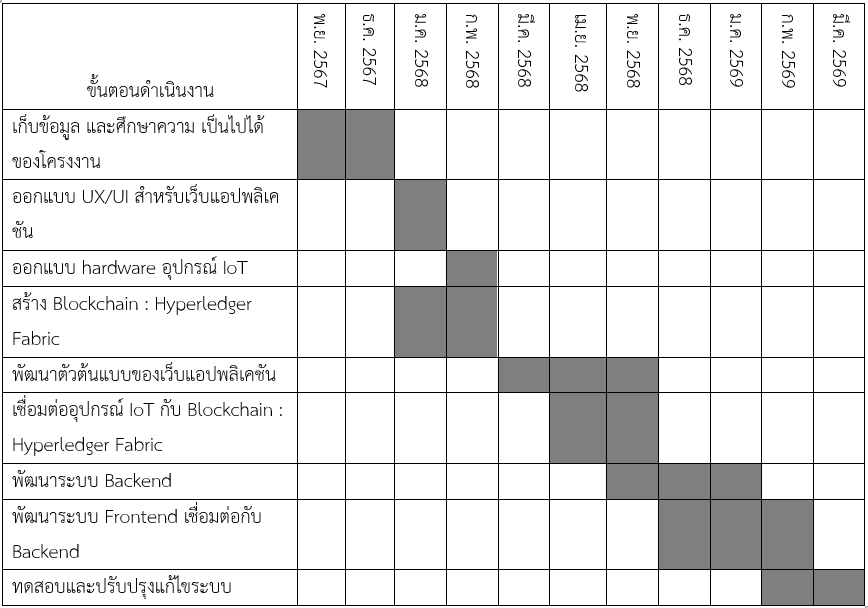
\includegraphics[width=\textwidth]{workplan.png}
    \caption{แผนการดำเนินงานโครงการ} 
\end{table}


\section{\ifenglish Roles and responsibilities\else บทบาทและความรับผิดชอบ\fi}
\begin{enumerate}
    \item นางสาวนันท์นภัส ศิริธนาโชคไพศาล: พัฒนาโครงสร้างส่วนหน้า (Frontend) สำหรับการใช้งานฟังก์ชันต่าง ๆ
    \begin{itemize}
        \item ออกแบบและพัฒนาส่วนติดต่อผู้ใช้ (User Interface) ให้ใช้งานได้สะดวกและเหมาะสม
        \item พัฒนาหน้าล็อกอินที่มีระบบตรวจสอบสิทธิ์ผู้ใช้ เพื่อให้สามารถเข้าถึงข้อมูลได้อย่างปลอดภัย
        \item สร้างระบบสำหรับการเข้าถึงและแสดงผลฟังก์ชันต่าง ๆ ภายในแอปพลิเคชัน เช่น การแสดงผลอุณหภูมิแบบเรียลไทม์ของสินค้าระหว่างการขนส่ง และการเพิ่มข้อมูลการจัดส่งสินค้า เพื่อให้สามารถติดตามสถานะของสินค้าได้อย่างแม่นยำ
        \item เชื่อมต่อโครงสร้างส่วนหน้า (Frontend) กับโครงสร้างส่วนหลัง (Backend) เพื่อให้ข้อมูลสามารถอัปเดตและแสดงผลแบบเรียลไทม์ รวมถึงพัฒนาอินเทอร์เฟซที่รองรับการแจ้งเตือนเมื่อเกิดความผิดปกติ
    \end{itemize}
    
    \item นายผืนป่า จำปาศรี: พัฒนาอุปกรณ์ตรวจจับอุณหภูมิ (Hardware)
    \begin{itemize}
        \item ออกแบบและพัฒนาอุปกรณ์เซ็นเซอร์ตรวจจับอุณหภูมิที่สามารถติดตั้งภายในระบบขนส่งสินค้า
        \item พัฒนาแบบจำลองการวิเคราะห์ข้อมูลอุณหภูมิ เพื่อประเมินความเสถียรของสภาพแวดล้อมระหว่างการขนส่ง และตรวจจับความผิดปกติที่อาจส่งผลต่อคุณภาพของอาหารแช่แข็ง
        \item ปรับปรุงอุปกรณ์ให้สามารถทำงานได้อย่างมีประสิทธิภาพภายใต้สภาพแวดล้อมที่
        หลากหลาย รวมถึงพัฒนาโหมดการทำงานที่ช่วยลดการใช้พลังงานในระหว่างการขนส่ง
        \item เชื่อมต่อเซ็นเซอร์เข้ากับระบบอินเทอร์เน็ตของสรรพสิ่ง (IoT) เพื่อให้ข้อมูลอุณหภูมิถูกบันทึกและส่งไปยังบล็อกเชน (Blockchain) ได้แบบเรียลไทม์
    \end{itemize}

    
    \item นางสาวปิ่นนารี พร้อมมิตร: พัฒนาโครงสร้างส่วนหลัง (Backend) การจัดสร้างบล็อกเชน (Blockchain) และการบริหารจัดการฐานข้อมูล
    \begin{itemize}
        \item ออกแบบและพัฒนาฐานข้อมูลกลาง เพื่อใช้ในการจัดเก็บข้อมูลอุณหภูมิ ข้อมูลการขนส่ง และผลการวิเคราะห์คุณภาพของสินค้า
        \item พัฒนาระบบโครงสร้างส่วนหลัง (Backend) ที่รองรับการประมวลผลข้อมูลแบบเรียลไทม์ และสามารถเชื่อมต่อกับอุปกรณ์อินเทอร์เน็ตของสรรพสิ่ง (IoT) เพื่อรับข้อมูลอุณหภูมิจากเซ็นเซอร์ที่ติดตั้งภายในระบบขนส่ง
        \item สร้างระบบบล็อกเชน (Blockchain) เพื่อใช้เป็นแพลตฟอร์มสำหรับการจัดเก็บข้อมูลอุณหภูมิและสถานะของสินค้าตลอดเส้นทางขนส่ง ซึ่งช่วยให้ข้อมูลมีความปลอดภัย ไม่สามารถเปลี่ยนแปลงหรือปลอมแปลงได้โดยไม่ได้รับอนุญาต
        \item พัฒนาระบบแจ้งเตือนอัตโนมัติ เมื่อมีการเปลี่ยนแปลงของอุณหภูมิที่อาจส่งผลกระทบต่อคุณภาพสินค้า โดยแจ้งเตือนไปยังผู้ที่เกี่ยวข้องเพื่อให้สามารถดำเนินการแก้ไขได้อย่างทันท่วงที
        \item 
    \end{itemize}
    
\end{enumerate}

\section{\ifenglish%
Impacts of this project on society, health, safety, legal, and cultural issues
\else%
ผลกระทบด้านสังคม สุขภาพ ความปลอดภัย กฎหมาย และวัฒนธรรม
\fi}

\subsection{ด้านสังคม}
โครงการนี้จะมีผลกระทบทางสังคมโดยการเพิ่มความโปร่งใสและการตรวจสอบย้อนกลับในกระบวนการขนส่งสินค้าที่ต้องควบคุมอุณหภูมิ เช่น อาหารแช่แข็ง ซึ่งส่งผลให้ผู้บริโภคได้รับสินค้าที่มีคุณภาพและปลอดภัยมากขึ้น การใช้เทคโนโลยีบล็อกเชน (Blockchain) ช่วยลดปัญหาการปลอมแปลงข้อมูล และเพิ่มความมั่นใจในระบบห่วงโซ่อุปทาน ซึ่งสามารถช่วยส่งเสริมการพัฒนาเศรษฐกิจในท้องถิ่นและยกระดับมาตรฐานของธุรกิจในภาคการขนส่งสินค้า

\subsection{ด้านสุขภาพ}
การควบคุมอุณหภูมิในการขนส่งอาหารแช่แข็งมีผลโดยตรงต่อสุขภาพของผู้บริโภค การใช้ระบบอินเทอร์เน็ตของสรรพสิ่ง (Internet of Things: IoT) เพื่อเฝ้าระวังอุณหภูมิอย่างต่อเนื่องจะช่วยลดโอกาสในการเกิดการปนเปื้อนหรือการเสื่อมสภาพของอาหาร ซึ่งสามารถป้องกันโรคที่เกิดจากอาหารที่ไม่ปลอดภัย รวมถึงลดความเสี่ยงจากการแพร่กระจายของโรคระบาดที่เกี่ยวข้องกับการรับประทานอาหาร

\subsection{ด้านความปลอดภัย}
โครงการนี้สามารถเพิ่มความปลอดภัยในการขนส่งอาหารแช่แข็งได้ ด้วยการติดตามสถานะของอุณหภูมิและสถานที่ขนส่งแบบเรียลไทม์ ผ่านเซ็นเซอร์ IoT และการตรวจสอบข้อมูลบนบล็อกเชน เมื่อมีการแจ้งเตือนความผิดปกติในอุณหภูมิหรือเส้นทางการขนส่ง จะสามารถดำเนินการแก้ไขได้ทันที เพื่อป้องกันความเสียหายของสินค้าและอันตรายที่อาจเกิดขึ้น

\subsection{ด้านกฎหมาย}
เทคโนโลยีบล็อกเชน (Blockchain) ช่วยให้สามารถบันทึกข้อมูลอย่างโปร่งใสและไม่สามารถแก้ไขได้โดยไม่ได้รับอนุญาต ซึ่งช่วยให้สามารถตรวจสอบการปฏิบัติตามกฎหมายและระเบียบข้อบังคับได้ง่ายขึ้น โดยเฉพาะในด้านการควบคุมการขนส่งสินค้าที่ต้องควบคุมอุณหภูมิ เช่น อาหารแช่แข็ง การบังคับใช้กฎหมายที่เกี่ยวข้องกับการขนส่งอาหารและสุขอนามัยจะมีประสิทธิภาพมากขึ้นเมื่อมีระบบการตรวจสอบที่ชัดเจน

\subsection{ด้านวัฒนธรรม}
การใช้เทคโนโลยีใหม่ๆ ในการขนส่งและควบคุมอุณหภูมิอาจมีผลต่อการเปลี่ยนแปลงวิธีการทำงานของภาคการขนส่ง โดยเฉพาะอย่างยิ่งในวัฒนธรรมองค์กรที่มุ่งเน้นการปรับปรุงและพัฒนาเทคโนโลยีใหม่ๆ การนำเทคโนโลยีเหล่านี้มาใช้สามารถกระตุ้นให้เกิดการยอมรับในนวัตกรรมใหม่ในสังคมไทย และเพิ่มขีดความสามารถในการแข่งขันในระดับสากล

\subsection{แนวทางและโยชน์ในการประยุกต์ใช้งานโครงงานกับงานในด้านอื่นๆ รวมถึงผลกระทบในด้านสังคมและสิ่งแวดล้อมจากการใช้ความรู้ทางวิศวกรรมที่ได้}
โครงงานนี้สามารถประยุกต์ใช้ในหลายด้าน เช่น
\begin{itemize}
    \item การขนส่งยา – การใช้ระบบบล็อกเชน (Blockchain) และ IoT เพื่อควบคุมอุณหภูมิและสถานะของยาในระหว่างการขนส่ง ทำให้มั่นใจได้ว่ายาที่มีความสำคัญจะไม่สูญเสียคุณภาพและไม่เสี่ยงต่อการถูกปลอมแปลง
    \item การขนส่งผลิตภัณฑ์ทางการแพทย์ – ผลิตภัณฑ์ทางการแพทย์ที่ต้องการการควบคุมอุณหภูมิ เช่น วัคซีนและอุปกรณ์ทางการแพทย์ สามารถได้รับประโยชน์จากระบบนี้
    \item การขนส่งสินค้าอุปโภคบริโภคอื่นๆ – ระบบนี้สามารถขยายไปใช้กับสินค้าประเภทอื่นๆ ที่ต้องการการควบคุมอุณหภูมิหรือสภาพแวดล้อมในการขนส่ง
\end{itemize}

ผลกระทบในด้านสังคมและสิ่งแวดล้อมจากการใช้ความรู้ทางวิศวกรรมที่ได้
จากการใช้เทคโนโลยี IoT และบล็อกเชน (Blockchain) ในการจัดการห่วงโซ่อุปทาน อาจช่วยลดการใช้พลังงานในการขนส่งและลดการปล่อยมลพิษจากการขนส่งที่ไม่เหมาะสม โดยการติดตามเส้นทางการขนส่งและสถานะของสินค้า ทำให้สามารถประหยัดทรัพยากรได้ นอกจากนี้ยังช่วยลดการสูญเสียสินค้าจากการขนส่งที่ผิดพลาด หรือไม่เป็นไปตามมาตรฐาน ซึ่งส่งผลดีต่อสิ่งแวดล้อมโดยการลดขยะและการสูญเสียทรัพยากร
